%!TEX root = ../main.tex
\chapter{Modelli matematici}

\LezioneS{22/02/2021}

Un modello matematico è un compromesso tra complessità del mondo reale e idee astratte della matematica. Li applicheremo spesso nel contesto della meccanica dei continui.

Ci serviranno due mattoni principali
\begin{itemize}
    \item leggi generali (conservazione, bilancio dell'energia, della massa, della carica)
    \item leggi costitutive, di natura sperimentale, costruite ad hoc per catturare la natura essenziale del fenomeno che osserviamo (di Fourier, di Fiek, di Ohm...)
\end{itemize}

Si perviene quindi a equazioni o sistemi di equazioni ordinarie o alle derivate parziali.

Una EDP è un'equazione della forma
\begin{equation*}
    F(\x,t,u,u_{t},u_{x_{j}},u_{x_{i} x_{j}},\dotsc)=0 \qquad \x\in \mathbb{R} ^{n}
\end{equation*}
L'ordine di un'equazione è l'ordine massimo di derivazione.

\section{Distinzione di EDP}
Si distinguono
\begin{itemize}
    \item equazioni lineari: $F$ è un polinomio di primo grado in $u$ e in tutte le derivate parziali
    \item equazioni non lineari
          \begin{itemize}
              \item semilineari: $F$ è non lineare solo rispetto ad $u$
              \item quasilineari: $F$ è lineare nelle derivate di ordine massimo, con coefficienti che possono dipendere da $u$ e dalle derivate di ordine inferiore
              \item completamente non lineari: $F$ è non lineare nelle derivate di ordine massimo
          \end{itemize}
\end{itemize}
\begin{definition}
    [Laplaciano] Definiamo il laplaciano di $\displaystyle u=u(x_{1},\dotsc,x_{n})$
    \begin{equation*}
        \Delta u=\sum ^{n}_{j=1}\frac{\partial ^{2} u}{{\partial x_{j}}^{2}}
    \end{equation*}
\end{definition}
\textit{Esempi.}
\begin{itemize}
    \item Lineare

          \textit{Calore o diffusione}

          \begin{equation*}
              u_{t} -D(x,t) \Delta u=f
          \end{equation*}

          \textit{Laplace/Poisson}

          \begin{equation*}
              \Delta u=f(x,t)
          \end{equation*}

          \textit{Onde}

          \begin{equation*}
              u_{tt} -c^{2} \Delta u=0\ \ \ c(x,t)
          \end{equation*}
    \item Non lineare
          \begin{itemize}
              \item Semilineare

                    \textit{Fisher-Kolmogorov}
                    \begin{equation*}
                        u_{t} -D\Delta u=f(u) =ru(1-u)
                    \end{equation*}
              \item Quasi lineare

                    \textit{Burgers}
                    \begin{equation*}
                        u_{t} +u\cdotp u_{x} =\varepsilon u_{xx} \ \ \ \ x\in \mathbb{R}
                    \end{equation*}

                    \textit{Equazione delle superfici minime (o delle bolle di sapone)}
                    \begin{equation*}
                        \mathrm{div}\left(\frac{\nabla u}{\sqrt{1+| \nabla u| ^{2}}}\right) =0
                    \end{equation*}
              \item Completamente non lineare

                    \textit{Iconale} (ottica geometrica)\footnote{$c(x)$ è l'indice di rifrazione.}
                    \begin{equation*}
                        | \nabla u| ^{2} =c(x)
                    \end{equation*}

                    \textit{Altro esempio di equazione completamente non lineare.}

                    Sia $u=u(x),x\in \mathbb{R}$, consideriamo un'equazione del secondo ordine lineare
                    \begin{equation*}
                        \mathcal{L} u=\sum ^{n}_{i,j=1} a_{ij}(x) u_{x_{i} x_{j}} =a_{11}(x) u_{x_{1} x_{1}} +\dotsc +a_{nn}(x) u_{x_{n} x_{n}}
                    \end{equation*}Prendo due operatori del tipo $\mathcal{L}_{1} u$ e $\mathcal{L}_{2} u$. Allora
                    \begin{equation*}
                        F(u)(x) =\max\{\mathcal{L}_{1} u(x),\mathcal{L}_{2} u(x)\}
                    \end{equation*}è completamente non lineare.
          \end{itemize}
\end{itemize}

Se è presente il tempo, si possono assegnare delle condizioni iniziali.
\section{Problema ben posto}

Compito dell'analisi teorica è, una volta costruito il modello consono, stabilire quale tipo di dati è necessario assegnare per ottenere
\begin{enumerate}
    \item \textbf{Esistenza}\\
          L'esistenza è un controllo di consistenza, perché il modello non è la realtà, ma cerca di copiarla.
          \begin{gather*}
              \mathrm{div}(\nabla u) =\Delta u=0\\
              \mathrm{div}(a(x) \nabla u) =\nabla a\cdotp \nabla u+a\Delta u
          \end{gather*}
          Voglio $u\in C^{2}$, ci sono problemi se esce un termine $a$ che tiene conto dell'anisotropia (discontinuità), perché $\nabla a$ non ha senso, essendo discontinuo.

    \item \textbf{Unicità}\\
          L'unicità è importante per l'approssimazione, vogliamo essere certi che ci sia un'unica soluzione a cui far tendere l'approssimazione.

    \item \textbf{Dipendenza continua dai dati}\\
          La dipendenza continua dai dati è importante perché è una forma di \textit{stabilità} rispetto all'argomento. In generale, siano $g_{1},g_{2}$ i dati di un problema e $u_{1},u_{2}$ le corrispondenti soluzioni. Vi è stabilità se
          \begin{equation*}
              \text{dist}(g_{1},g_{2})\rightarrow 0\ \ \Rightarrow \ \ \text{dist}(u_{1},u_{2})\rightarrow 0
          \end{equation*}
\end{enumerate}

Un problema di questo tipo è un problema ben posto \textit{secondo Hadamard.}.

Non abbiamo ancora definito quale distanza utilizzare, ricordiamone alcune per il momento. Supponiamo che $g_{1},g_{2}$ siano due funzioni definite su una certa regione in $R\subseteq \mathbb{R}^{n}$.
\begin{itemize}
    \item norma infinito
          \begin{equation*}
              \Vert g_{1} -g_{2}\Vert _{L^{\infty }(R)} =\sup _{x\in R}| g_{1}(x) -g_{2}(x)|
          \end{equation*}
    \item media quadratica
          \begin{equation*}
              \left(\frac{1}{| R| }\int _{R}| g_{1}(x) -g_{2}(x)| ^{2} \dx\right)^{1/2}
          \end{equation*}
\end{itemize}

L'obiettivo delle prossime lezioni è guardare un'equazione del tipo
\begin{equation*}
    u_{t} -D\Delta u+\mathbf{v} \cdotp \nabla u+ru=f(x,t)
\end{equation*}
e dedurre subito che
\begin{itemize}
    \item il primo è un tasso di variazione di $u$ nel tempo
    \item il secondo è un termine di diffusione
    \item il terzo è trasporto
    \item il quarto è una reazione o decadimento
    \item l'ultimo è una sorgente esogena
\end{itemize}

\LezioneS{23/02/2021}
\section{Topologia di \texorpdfstring{$\mathbb{R}^{n}$}{Rn}}
\begin{definition}
    [Palla aperta] Definiamo il concetto generale di intorno \textbf{aperto}, di raggio $r$ centrato in $\x$
    \begin{equation*}
        B_{r}(\x) =\left\{\y\in \mathbb{R}^{n} :| \y-\x| < r\right\}
    \end{equation*}
\end{definition}
Sia $E\subseteq \mathbb{R}^{n}$, $\x\in \mathbb{R}^{n}$ si dice
\begin{itemize}
    \item \textbf{punto interno} ad $E$ se $\x\in E$ ed esiste una sfera tale che $B_{r}(\x) \subset E$
    \item \textbf{punto esterno} ad $E$ se esiste una sfera $B_{r}(\x) \subset \mathbb{R}^{n} \setminus E$
    \item \textbf{punto di frontiera} per $E$ se \textbf{ogni} sfera $B_{r}(\x)$ contiene punti di $E$ e del complementare. I punti di frontiera possono appartenere ad $E$ o meno.
\end{itemize}

\begin{figure}[htpb]
    \centering


    \tikzset{every picture/.style={line width=0.75pt}} %set default line width to 0.75pt        

    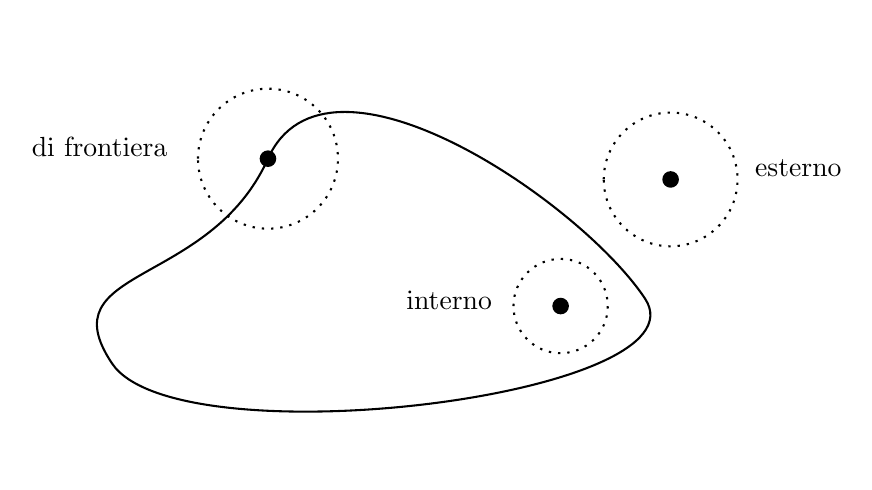
\begin{tikzpicture}[x=0.75pt,y=0.75pt,yscale=-1,xscale=1]
        %uncomment if require: \path (0,175); %set diagram left start at 0, and has height of 175

        %Shape: Polygon Curved [id:ds2940079142194729] 
        \draw   (98.63,138.34) .. controls (67.31,91.38) and (145.59,102.34) .. (173.77,39.71) .. controls (201.95,-22.91) and (324.07,60.06) .. (355.38,107.03) .. controls (386.69,154) and (129.94,185.31) .. (98.63,138.34) -- cycle ;
        %Shape: Circle [id:dp7776467971754304] 
        \draw  [dash pattern={on 0.84pt off 2.51pt}] (140.05,39.71) .. controls (140.05,21.09) and (155.15,5.99) .. (173.77,5.99) .. controls (192.4,5.99) and (207.5,21.09) .. (207.5,39.71) .. controls (207.5,58.34) and (192.4,73.44) .. (173.77,73.44) .. controls (155.15,73.44) and (140.05,58.34) .. (140.05,39.71) -- cycle ;
        %Shape: Circle [id:dp3616124142040644] 
        \draw  [draw opacity=0][fill={rgb, 255:red, 0; green, 0; blue, 0 }  ,fill opacity=1 ] (169.77,39.71) .. controls (169.77,37.5) and (171.56,35.71) .. (173.77,35.71) .. controls (175.98,35.71) and (177.77,37.5) .. (177.77,39.71) .. controls (177.77,41.92) and (175.98,43.71) .. (173.77,43.71) .. controls (171.56,43.71) and (169.77,41.92) .. (169.77,39.71) -- cycle ;

        %Shape: Circle [id:dp507315348623798] 
        \draw  [dash pattern={on 0.84pt off 2.51pt}] (335.55,49.71) .. controls (335.55,31.91) and (349.98,17.49) .. (367.77,17.49) .. controls (385.57,17.49) and (400,31.91) .. (400,49.71) .. controls (400,67.51) and (385.57,81.94) .. (367.77,81.94) .. controls (349.98,81.94) and (335.55,67.51) .. (335.55,49.71) -- cycle ;
        %Shape: Circle [id:dp9744198261464871] 
        \draw  [draw opacity=0][fill={rgb, 255:red, 0; green, 0; blue, 0 }  ,fill opacity=1 ] (363.77,49.71) .. controls (363.77,47.5) and (365.56,45.71) .. (367.77,45.71) .. controls (369.98,45.71) and (371.77,47.5) .. (371.77,49.71) .. controls (371.77,51.92) and (369.98,53.71) .. (367.77,53.71) .. controls (365.56,53.71) and (363.77,51.92) .. (363.77,49.71) -- cycle ;
        %Shape: Circle [id:dp6478352052119392] 
        \draw  [dash pattern={on 0.84pt off 2.51pt}] (292.05,110.71) .. controls (292.05,98.16) and (302.22,87.99) .. (314.77,87.99) .. controls (327.33,87.99) and (337.5,98.16) .. (337.5,110.71) .. controls (337.5,123.26) and (327.33,133.44) .. (314.77,133.44) .. controls (302.22,133.44) and (292.05,123.26) .. (292.05,110.71) -- cycle ;
        %Shape: Circle [id:dp6783224607477678] 
        \draw  [draw opacity=0][fill={rgb, 255:red, 0; green, 0; blue, 0 }  ,fill opacity=1 ] (310.77,110.71) .. controls (310.77,108.5) and (312.56,106.71) .. (314.77,106.71) .. controls (316.98,106.71) and (318.77,108.5) .. (318.77,110.71) .. controls (318.77,112.92) and (316.98,114.71) .. (314.77,114.71) .. controls (312.56,114.71) and (310.77,112.92) .. (310.77,110.71) -- cycle ;

        % Text Node
        \draw (239,102) node [anchor=north west][inner sep=0.75pt]   [align=left] {interno};
        % Text Node
        \draw (58.5,28) node [anchor=north west][inner sep=0.75pt]   [align=left] {di frontiera};
        % Text Node
        \draw (407,38.5) node [anchor=north west][inner sep=0.75pt]   [align=left] {esterno};

    \end{tikzpicture}
\end{figure}
\FloatBarrier

Inoltre
\begin{itemize}
    \item $\x$ è \textbf{punto limite o di accumulazione} per $E$ se $\forall B_{r}(\x)$ contiene $\infty $ punti di $E$. Equivalentemente: se $\exists \{\x_{k}\} \subset E:\x_{k}\rightarrow \x$ per $k\rightarrow +\infty$.
    \item Un punto che non è di accumulazione è un \textbf{punto isolato.}
\end{itemize}

Sia $E\subseteq \mathbb{R}^{n}$, $E$ si dice
\begin{itemize}
    \item \textbf{aperto} se $\forall \x\in E$, $\x$ è interno ad $E$\footnote{per esempio $B_{r}(\x)$ è un aperto.}
          \begin{itemize}
              \item Un aperto $E$ si dice \textbf{connesso} se non si può scrivere come unione di due aperti non vuoti e disgiunti, oppure se esiste una curva contenuta nell'insieme che congiunge tutti i punti.

                    Chiameremo \textbf{dominio} un aperto connesso.
          \end{itemize}
    \item \textbf{chiuso} se $\mathbb{R}^{n} \setminus E$ è aperto, oppure se contiene tutti i propri punti di frontiera $\partial E\subseteq E$, oppure se contiene tutti i propri punti limite.
    \item si dice \textbf{chiusura} di $E$ l'insieme $\displaystyle \overline{E} =\partial E\cup E$
    \item si dice \textbf{convesso} se $\forall x,y\in E$ il segmento che li congiunge è contenuto nell'insieme
          \begin{equation*}
              [ x,y] =\{tx+(1-t) y,0\leqslant t\leqslant 1\} \subseteq E
          \end{equation*}Un insieme convesso è automaticamente connesso, ma non in generale il contrario.
          \begin{figure}[htpb]
              \centering


              \tikzset{every picture/.style={line width=0.75pt}} %set default line width to 0.75pt        

              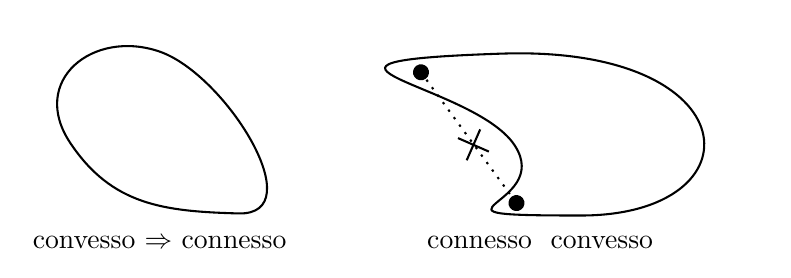
\begin{tikzpicture}[x=0.75pt,y=0.75pt,yscale=-1,xscale=1]
                  %uncomment if require: \path (0,133); %set diagram left start at 0, and has height of 133

                  %Shape: Polygon Curved [id:ds38185510936846945] 
                  \draw   (283,16.55) .. controls (403,12.55) and (408,94.55) .. (321,94.55) .. controls (234,94.55) and (309,90.55) .. (289,60.55) .. controls (269,30.55) and (163,20.55) .. (283,16.55) -- cycle ;
                  %Shape: Polygon Curved [id:ds8879242849839888] 
                  \draw   (118,15.55) .. controls (150,26.55) and (192,94.55) .. (156,93.55) .. controls (120,92.55) and (95,89.55) .. (75,59.55) .. controls (55,29.55) and (86,4.55) .. (118,15.55) -- cycle ;
                  %Straight Lines [id:da8125811443764148] 
                  \draw  [dash pattern={on 0.84pt off 2.51pt}]  (244,25.55) -- (290,88.55) ;
                  \draw [shift={(290,88.55)}, rotate = 53.86] [color={rgb, 255:red, 0; green, 0; blue, 0 }  ][fill={rgb, 255:red, 0; green, 0; blue, 0 }  ][line width=0.75]      (0, 0) circle [x radius= 3.35, y radius= 3.35]   ;
                  \draw [shift={(244,25.55)}, rotate = 53.86] [color={rgb, 255:red, 0; green, 0; blue, 0 }  ][fill={rgb, 255:red, 0; green, 0; blue, 0 }  ][line width=0.75]      (0, 0) circle [x radius= 3.35, y radius= 3.35]   ;
                  \draw   (261.83,57.25) -- (276.71,63.75)(272.52,53.06) -- (266.02,67.94) ;

                  % Text Node
                  \draw (55.5,103) node [anchor=north west][inner sep=0.75pt]   [align=left] {convesso $\displaystyle \Rightarrow $ connesso};
                  % Text Node
                  \draw (245.5,103) node [anchor=north west][inner sep=0.75pt]   [align=left] {connesso $\displaystyle \nRightarrow $ convesso};

              \end{tikzpicture}
              \caption{Controesempio insieme connesso che non implica convesso.}
          \end{figure}
          \FloatBarrier
    \item si dice \textbf{compatto} se da \textit{qualunque} copertura aperta di $E$ si può estrarre una sottocopertura finita.\footnote{In $\mathbb{R}^{n}$ vale l'implicazione: compatto $\Leftrightarrow$ chiuso e limitato.}
    \item si dice \textbf{limitato} se esiste una sfera $B_{r}(0)$ che contiene $E$, cioè se $\exists B_{r}(0) :E\subset B_{r}(0)$
\end{itemize}
\begin{nb}
    $\mathbb{R}^{n}$ è sia aperto che chiuso, ma allora anche il suo complementare, l'insieme vuoto, lo è. Sono gli unici due insiemi in $\mathbb{R}^{n}$ che lo sono.
\end{nb}
\begin{definition}
    [Copertura] Una famiglia $\mathcal{F}$ di aperti si dice copertura di $E$ se
    \begin{equation*}
        \bigcup _{A\in \mathcal{F}} A\supset E
    \end{equation*}
\end{definition}

\begin{figure}[htpb]
    \centering


    \tikzset{every picture/.style={line width=0.75pt}} %set default line width to 0.75pt        

    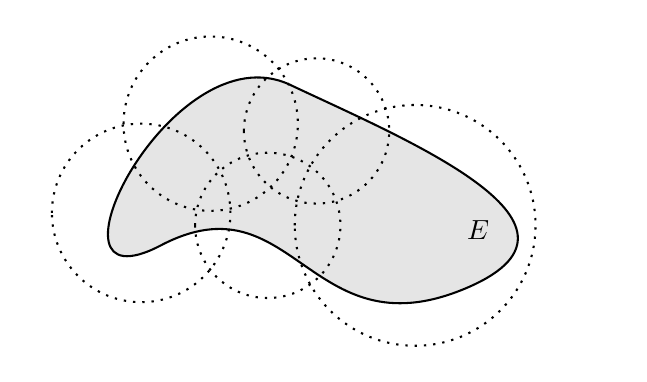
\begin{tikzpicture}[x=0.75pt,y=0.75pt,yscale=-1,xscale=1]
        %uncomment if require: \path (0,300); %set diagram left start at 0, and has height of 300

        %Shape: Polygon Curved [id:ds4561603116600126] 
        \draw  [fill={rgb, 255:red, 0; green, 0; blue, 0 }  ,fill opacity=0.1 ] (233.71,42.76) .. controls (290.91,69.78) and (391.44,111.01) .. (317.12,141.35) .. controls (242.81,171.68) and (235.22,86.75) .. (171.52,120.12) .. controls (107.82,153.48) and (176.5,15.75) .. (233.71,42.76) -- cycle ;
        %Shape: Circle [id:dp28763635934544385] 
        \draw  [dash pattern={on 0.84pt off 2.51pt}] (119,104.5) .. controls (119,80.75) and (138.25,61.5) .. (162,61.5) .. controls (185.75,61.5) and (205,80.75) .. (205,104.5) .. controls (205,128.25) and (185.75,147.5) .. (162,147.5) .. controls (138.25,147.5) and (119,128.25) .. (119,104.5) -- cycle ;
        %Shape: Circle [id:dp6205183942199646] 
        \draw  [dash pattern={on 0.84pt off 2.51pt}] (153.5,61.5) .. controls (153.5,38.3) and (172.3,19.5) .. (195.5,19.5) .. controls (218.7,19.5) and (237.5,38.3) .. (237.5,61.5) .. controls (237.5,84.7) and (218.7,103.5) .. (195.5,103.5) .. controls (172.3,103.5) and (153.5,84.7) .. (153.5,61.5) -- cycle ;
        %Shape: Circle [id:dp17944962123684904] 
        \draw  [dash pattern={on 0.84pt off 2.51pt}] (236,110.5) .. controls (236,78.47) and (261.97,52.5) .. (294,52.5) .. controls (326.03,52.5) and (352,78.47) .. (352,110.5) .. controls (352,142.53) and (326.03,168.5) .. (294,168.5) .. controls (261.97,168.5) and (236,142.53) .. (236,110.5) -- cycle ;
        %Shape: Circle [id:dp707943242370255] 
        \draw  [dash pattern={on 0.84pt off 2.51pt}] (211.5,65) .. controls (211.5,45.67) and (227.17,30) .. (246.5,30) .. controls (265.83,30) and (281.5,45.67) .. (281.5,65) .. controls (281.5,84.33) and (265.83,100) .. (246.5,100) .. controls (227.17,100) and (211.5,84.33) .. (211.5,65) -- cycle ;
        %Shape: Circle [id:dp9199082293705505] 
        \draw  [dash pattern={on 0.84pt off 2.51pt}] (188,110.5) .. controls (188,91.17) and (203.67,75.5) .. (223,75.5) .. controls (242.33,75.5) and (258,91.17) .. (258,110.5) .. controls (258,129.83) and (242.33,145.5) .. (223,145.5) .. controls (203.67,145.5) and (188,129.83) .. (188,110.5) -- cycle ;

        % Text Node
        \draw (317.5,106.9) node [anchor=north west][inner sep=0.75pt]    {$E$};
    \end{tikzpicture}
    \caption{Copertura di un insieme in due dimensioni.}
\end{figure}

\textit{Esempio.}

Tipici esempi di compatti sono gli intervalli \textbf{chiusi} e \textbf{limitati} in $\mathbb{R}$
\begin{equation*}
    E=[ a,b] \subset \mathbb{R}
\end{equation*}
\textit{Controesempio.}

Se consideriamo $E=(0,1]$ non è chiuso. Consideriamo la famiglia di aperti
\begin{equation*}
    A_{k} =\left(\frac{1}{k},1+\frac{1}{k}\right),k=1,2,\dotsc \ \ \Rightarrow \ \ \bigcup ^{\infty }_{k=1} A_{k} \supset E
\end{equation*}
Tuttavia non riesco a estrarre nessuna sottocopertura \textit{finita}, perché lascerei fuori degli elementi vicino all'origine.
\section{Topologia indotta}

Sia $X$ un insieme. Introdurre una topologia in $X$ significa introdurre una famiglia $\mathcal{A}$, i cui elementi saranno \textbf{aperti}, con le seguenti proprietà
\begin{itemize}
    \item $X$ e $\emptyset $ appartengono ad $\mathcal{A}$
    \item Unione di un numero \textbf{finito o infinito} di aperti di $\mathcal{A}$ è ancora un elemento di $\mathcal{A}$
    \item Intersezione di un numero \textbf{finito} di aperti di $\mathcal{A}$ è ancora un elemento di $\mathcal{A}$
\end{itemize}

\textit{Controesempio. }

Un'intersezione infinita di aperti può essere un insieme chiuso:
\begin{gather*}
    C_{k} =\left\{(x,y) \in \mathbb{R}^{2} :x^{2} +y^{2} < 1+\frac{1}{k}\right\}\\
    \\
    \bigcap\limits ^{\infty }_{k=1} C_{k} =\left\{x^{2} +y^{2} \leqslant 1\right\} \ \text{chiuso!}
\end{gather*}
\begin{figure}[htpb]
    \centering


    \tikzset{every picture/.style={line width=0.75pt}} %set default line width to 0.75pt        

    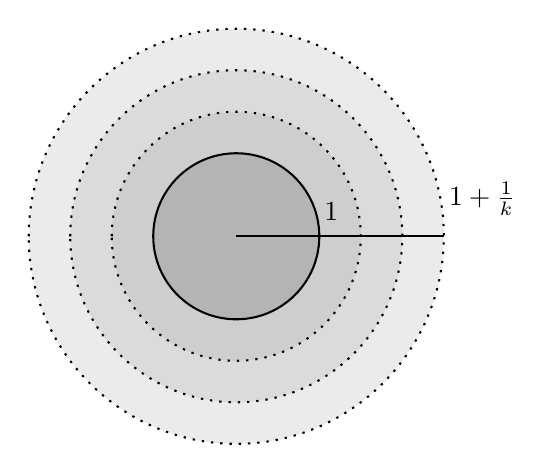
\begin{tikzpicture}[x=0.75pt,y=0.75pt,yscale=-1,xscale=1]
        %uncomment if require: \path (0,218); %set diagram left start at 0, and has height of 218

        %Shape: Circle [id:dp9214987751630181] 
        \draw  [fill={rgb, 255:red, 155; green, 155; blue, 155 }  ,fill opacity=0.2 ][dash pattern={on 0.84pt off 2.51pt}] (130,110) .. controls (130,54.77) and (174.77,10) .. (230,10) .. controls (285.23,10) and (330,54.77) .. (330,110) .. controls (330,165.23) and (285.23,210) .. (230,210) .. controls (174.77,210) and (130,165.23) .. (130,110) -- cycle ;
        %Shape: Circle [id:dp7587137498598324] 
        \draw  [fill={rgb, 255:red, 155; green, 155; blue, 155 }  ,fill opacity=0.2 ][dash pattern={on 0.84pt off 2.51pt}] (150,110) .. controls (150,65.82) and (185.82,30) .. (230,30) .. controls (274.18,30) and (310,65.82) .. (310,110) .. controls (310,154.18) and (274.18,190) .. (230,190) .. controls (185.82,190) and (150,154.18) .. (150,110) -- cycle ;
        %Shape: Circle [id:dp9171220969714382] 
        \draw  [fill={rgb, 255:red, 155; green, 155; blue, 155 }  ,fill opacity=0.2 ][dash pattern={on 0.84pt off 2.51pt}] (170,110) .. controls (170,76.86) and (196.86,50) .. (230,50) .. controls (263.14,50) and (290,76.86) .. (290,110) .. controls (290,143.14) and (263.14,170) .. (230,170) .. controls (196.86,170) and (170,143.14) .. (170,110) -- cycle ;
        %Shape: Circle [id:dp4072549012269078] 
        \draw  [fill={rgb, 255:red, 155; green, 155; blue, 155 }  ,fill opacity=0.5 ] (190,110) .. controls (190,87.91) and (207.91,70) .. (230,70) .. controls (252.09,70) and (270,87.91) .. (270,110) .. controls (270,132.09) and (252.09,150) .. (230,150) .. controls (207.91,150) and (190,132.09) .. (190,110) -- cycle ;
        %Straight Lines [id:da14227929179339527] 
        \draw    (230,110) -- (330,110) ;

        % Text Node
        \draw (271,92.4) node [anchor=north west][inner sep=0.75pt]    {$1$};
        % Text Node
        \draw (331,82.4) node [anchor=north west][inner sep=0.75pt]    {$1+\frac{1}{k}$};

    \end{tikzpicture}
    \caption{Intersezione infinita di aperti che è un insieme chiuso.}
\end{figure}
\FloatBarrier

\begin{definition}
    [Insieme aperto rispetto a topologia indotta] Sia $\Omega $ dominio di $\mathbb{R}^{n}$ con bordo $\partial \Omega $. Si dice che $\displaystyle A\subset \partial \Omega $ è aperto relativamente a $\displaystyle \partial \Omega $, rispetto alla topologia indotta da $\displaystyle \mathbb{R}^{n}$, se $\exists $ un aperto $E$ di $\mathbb{R}^{n}$ tale che $A=E\cap \partial \Omega $
\end{definition}
\begin{figure}[htpb]
    \centering


    \tikzset{every picture/.style={line width=0.75pt}} %set default line width to 0.75pt        

    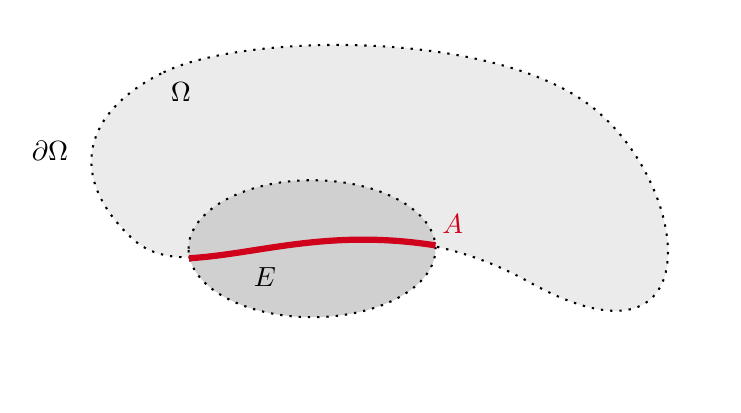
\begin{tikzpicture}[x=0.75pt,y=0.75pt,yscale=-1,xscale=1]
        %uncomment if require: \path (0,163); %set diagram left start at 0, and has height of 163

        %Shape: Polygon Curved [id:ds7654783928439228] 
        \draw  [fill={rgb, 255:red, 155; green, 155; blue, 155 }  ,fill opacity=0.2 ][dash pattern={on 0.84pt off 2.51pt}] (170,27.8) .. controls (209,8.8) and (331,6.8) .. (378,45.8) .. controls (425,84.8) and (434,177.8) .. (346,128.8) .. controls (258,79.8) and (187,137.8) .. (155,108) .. controls (123,78.2) and (131,46.8) .. (170,27.8) -- cycle ;
        %Shape: Ellipse [id:dp3156933907308139] 
        \draw  [fill={rgb, 255:red, 208; green, 208; blue, 208 }  ,fill opacity=1 ][dash pattern={on 0.84pt off 2.51pt}] (182,112.8) .. controls (182,94.57) and (208.64,79.8) .. (241.5,79.8) .. controls (274.36,79.8) and (301,94.57) .. (301,112.8) .. controls (301,131.02) and (274.36,145.8) .. (241.5,145.8) .. controls (208.64,145.8) and (182,131.02) .. (182,112.8) -- cycle ;
        %Curve Lines [id:da32528948967523075] 
        \draw [color={rgb, 255:red, 208; green, 2; blue, 27 }  ,draw opacity=1 ][line width=2.25]    (182.2,117.4) .. controls (215.8,115.4) and (249,103) .. (301,111.2) ;

        % Text Node
        \draw (172,31.2) node [anchor=north west][inner sep=0.75pt]    {$\Omega $};
        % Text Node
        \draw (105,59.4) node [anchor=north west][inner sep=0.75pt]    {$\partial \Omega $};
        % Text Node
        \draw (212,120.4) node [anchor=north west][inner sep=0.75pt]    {$E$};
        % Text Node
        \draw (302.8,94.8) node [anchor=north west][inner sep=0.75pt]  [color={rgb, 255:red, 208; green, 2; blue, 27 }  ,opacity=1 ]  {$A$};

    \end{tikzpicture}
    \caption{Esempio di topologia indotta secondo la definizione.}
\end{figure}
\FloatBarrier

\textit{Esempio.}

$X=[ -1,1] \subset \mathbb{R}$

L'insieme $A=(-1,1]$ lo posso vedere come $\subset \mathbb{R}$ o come $\subset X$. Relativamente a $\displaystyle \mathbb{R}$ non è né aperto né chiuso. Nel secondo caso lo posso scrivere come
\begin{equation*}
    \underbrace{(-1,1]}_{A} = \underbrace{[-1,1]}_{X} \cap \underbrace{(-1,2)}_{E}
\end{equation*}
In questo caso $X$ ricopre il ruolo di $\partial\Omega$, infatti in realtà non serve che sia il bordo di un dominio, basta che sia aperto (o chiuso se stiamo dando la definizione complementare). Naturalmente di $E$ ci basta che ne esista almeno uno, potevamo prenderne anche un diverso, non c'è nulla di speciale nel $2$ all'estremo destro, l'importante era che fosse a destra di $1$.

Quindi è un \textit{aperto relativamente a X, rispetto alla topologia indotta da }$\displaystyle \mathbb{R}$!
\section{Ripasso di Analisi 2 e 3}

\textbf{Serie di funzioni}

Sia $\Omega \subseteq \mathbb{R}^{n}$, data una successione di funzioni $\displaystyle f_{k} :\Omega \rightarrow \mathbb{R}$, definiamo:
\begin{equation*}
    S_{N}(x) =\sum\limits ^{N}_{k=1} f_{k}(x) \qquad S(x) = \lim_{N \to \infty} S_{N}(x) =\sum\limits ^{\infty }_{k=1} f_{k}(x)
\end{equation*}
\begin{itemize}
    \item \textbf{Convergenza uniforme} di una serie di funzioni:

          $\sum f_{k}$ converge uniformemente in $\Omega $ se \begin{equation*}
              \sup _{\Omega }| S_{N}(x) -S(x)| \rightarrow 0,\ N\rightarrow +\infty
          \end{equation*}
    \item \textbf{Test di Weierstrass} (condizione sufficiente per la convergenza uniforme):

          Se $\forall k\geqslant 1$ esiste $a_{k}$ tale che
          \begin{equation*}
              | f_{k}(x)| \leqslant a_{k} \ \forall x\in \Omega \ \ \land \ \ \sum\limits ^{\infty }_{k=1} a_{k} < \infty
          \end{equation*}

          $\Rightarrow \sum f_{k}$ converge uniformemente in $\Omega $

    \item \textbf{Scambio serie e limite:}

          Se $\sum f_{k}$ converge uniformemente in $\Omega $ e $f_{k}$, $k\geqslant 1$, è continua in $\Omega $, allora $S$ è continua in $\Omega $ e
          \begin{equation*}
              x_{0} \in \Omega \ \ \lim\limits _{x\rightarrow x_{0}}\sum f_{k}(x) =\sum f_{k}(x_{0})
          \end{equation*}

    \item \textbf{Scambio serie e derivata:}

          Siano $f_{k}$ derivabili in $\Omega$ per ogni $k\geqslant 1$, rispetto a $x_{j}$ se inoltre:
          \begin{itemize}
              \item esiste almeno un $x_{0} \in \Omega :\sum^{\infty }_{k=1} f_{k}(x_{0})$ è convergente, chiamiamo $F(x)$ la funzione a cui converge;
              \item $\sum^{\infty }_{k=1} \frac{\partial f_{k}(x)}{\partial x_{j}}$ è uniformemente convergente a una certa $f(x)$.
          \end{itemize}

          Allora per tutti gli $x\in \Omega$
          \begin{equation*}
              \frac{\partial }{\partial x_{j}} \underbrace{\sum^{\infty }_{k=1} f_{k}(x)}_{F(x)} = \underbrace{\sum^{\infty }_{k=1} \frac{\partial f_{k}(x)}{\partial x_{j}}}_{f(x)}
          \end{equation*}
\end{itemize}

\textbf{Integrali}
\begin{itemize}
    \item \textbf{Disuguaglianza di Holder}
          \begin{equation*}
              \left| \int _{\Omega } fg\right| \leqslant \left(\int _{\Omega }| f| ^{p}\right)^{1/p}\left(\int _{\Omega }| g| ^{q}\right)^{1/q}
          \end{equation*}

          dove \begin{equation*}
              \frac{1}{p} +\frac{1}{q} =1\ \ \ p,q\geqslant 1
          \end{equation*}
    \item \textbf{Disuguaglianza di Schwarz (}se $p=2=q$) \begin{equation*}
              \left| \int _{\Omega } fg\right| \leqslant \left(\int _{\Omega } f^{2}\right)^{1/2}\left(\int _{\Omega } g^{2}\right)^{1/2}
          \end{equation*}
\end{itemize}

\textbf{Funzioni}
Sia $\Omega \subseteq \mathbb{R}^{n}$. Definisco:
\begin{itemize}
    \item $C(\Omega)$, l'insieme delle \textbf{funzioni continue} in $\Omega $.
    \item $C(\overline{\Omega }) \subset C(\Omega)$, l'insieme delle \textbf{funzioni estendibili con continuità fino al bordo di} $\Omega $. Se $\Omega $ è limitato, $\overline{\Omega }$ è compatto.
    \item $C(\overline{\Omega })$ è uno spazio di Banach rispetto alla norma $\Vert g\Vert _{C(\overline{\Omega })} =\ \max_{\overline{\Omega }}| g| $
\end{itemize}

Posso estendere le definizioni a ordini di derivazione maggiori:
\begin{itemize}
    \item $C^{1}(\Omega) \dotsc C^{k}(\Omega)$, $k$ ordine di derivazione.
    \item Per $C^{1}(\overline{\Omega }) \dotsc C^{k}(\overline{\Omega })$ tutte le derivate fino alla $k$-esima sono estendibili con continuità fino al bordo di $\displaystyle \Omega $.
\end{itemize}

Definisco le norme per gli spazi $L^{p},1\leqslant p\leqslant +\infty $

\begin{equation*}
    \begin{array}{ l l }
        \Vert f\Vert _{L^{1}(\Omega)} =\int _{\Omega }| f|                            & \ \ \ \ p=1    \\
        \Vert f\Vert _{L^{p}(\Omega)} =\left(\int _{\Omega }| f| ^{p}\right)^{1/p} \  & \ 1< p< \infty \\
        \Vert f\Vert _{L^{\infty }(\Omega)} =\sup\limits _{\Omega }| f|               & \ \ \ p=\infty
    \end{array}
\end{equation*}
Gli spazi $\displaystyle L^{p}$ sono spazi di Banach, $\displaystyle L^{2}$ è anche di Hilbert.

\section{Domini regolari e Lipschitziani}

Avremo bisogno di classificare i domini $\Omega $ in $\mathbb{R}^{n}$ secondo il grado di regolarità della loro frontiera.

Possiamo descrivere il pezzo di bordo dentro la sferetta tramite un grafico cartesiano del tipo $y_{2} =\varphi (y_{1})$. Se il grafico è sufficientemente liscio, quella $\varphi $ sarà almeno $C^{1}$. Se la funzione è $C^{k}$ diremo che il dominio è di classe $C^{k}$, ovviamente per ogni punto del bordo.

\fg{0.7}{dominio-regolare}

\begin{definition}
    Un dominio $\Omega $ si dice di classe $C^{1}$ se per ogni punto $p\in \partial \Omega $ esiste un sistema di assi cartesiani $(y',y_{n}),y'\in \mathbb{R}^{n-1},y_{n} \in \mathbb{R}$, con origine in $p$, una sfera $B(p)$, una funzione $\varphi _{p}$ definita in un intorno $\mathcal{N}_{p} \subset \mathbb{R}^{n-1}$ di $y'=0'$, tale che
    \begin{equation*}
        \varphi _{p} \in C^{1}(\mathcal{N}_{p}),\ \varphi (0') =0
    \end{equation*}
    e che
    \begin{enumerate}
        \item $\partial \Omega \cap B(p) =\{(y',y_{n}) :y_{n} =\varphi _{p}(y'),y'\in \mathcal{N}_{p}\}$

              cioè il bordo coincide col grafico della funzione
        \item $\Omega \cap B(p) =\{(y',y_{n}) :y_{n}  >\varphi _{p}(y'),y'\in \mathcal{N}_{p}\}$

              cioè l'insieme sta tutto da una parte del grafico
    \end{enumerate}
\end{definition}

Le coppie $(\varphi,\mathcal{N})$ sono dette \textbf{carte locali}.

Se $\Omega $ è \textbf{limitato}, può essere descritto da un numero finito di carte locali $(\varphi _{p},\mathcal{N}_{p})$.

Se $\varphi _{p}$ è Lipschitziana il dominio si dice \textbf{dominio Lipschitziano.}
\begin{definition}
    [Funzione Lipschitziana] Una funzione $u:\Omega \rightarrow \mathbb{R}^{n}$ è Lipschitziana se
    \begin{equation*}
        | u(\x) -u(\y)| \leqslant L|\x-\y|,\ \ \forall \x,\y\in \Omega
    \end{equation*}
\end{definition}
Poiché il grafico di una funzione Lipschiziana può presentare angoli e/o spigoli, non ci si può aspettare l’esistenza di un iperpiano tangente in ogni suo punto. Tuttavia, l’insieme dei punti ``irregolari'' costituisce un insieme di misura nulla (secondo Lebesgue). Precisamente, vale il seguente teorema.
\begin{theorem}
    [di Rademacher] Se $f$ è lipschitziana in $\mathbb{R}^{n} \Rightarrow f$ è differenziabile q.o. in $\mathbb{R}^{n}$.
\end{theorem}
\section{Formule di integrazione per parti}

Sia $\Omega $ di classe $C^{1}$. Consideriamo una funzione vettoriale $\mathbf{F}:\mathbb{R}^{n}\to\mathbb{R}^{m}$. Vale il teorema della divergenza
\begin{equation*}
    \int _{\Omega }\mathrm{div}\mathbf{G}\dxx=\int _{\partial \Omega }\mathbf{G} \cdotp \nuu\dsig \qquad \text{dove}\ \nuu\ \text{è il versore normale.}
\end{equation*}
Sia $v$ una funzione scalare scalare $v:\mathbb{R}^{n}\to \mathbb{R}$, vale la regola di derivazione di Leibniz estesa a più dimensioni:
\begin{equation*}
    \mathrm{div}(v\mathbf{F}) =v\ \mathrm{div}(\mathbf{F}) +\nabla v\cdotp \mathbf{F}
\end{equation*}
da cui ricaviamo
\begin{equation*}
    v\ \mathrm{div}(\mathbf{F}) = \mathrm{div}(v\mathbf{F}) -\nabla v\cdotp \mathbf{F}
\end{equation*}
Integrando e applicando il teorema della divergenza otteniamo una \textbf{formula di integrazione per parti} in $\mathbb{R}^{n}$
\begin{equation}
    \boxed{\int _{\Omega } v\ \mathrm{div}(\mathbf{F}) \dxx = \int _{\partial \Omega } v\mathbf{F} \cdotp \nuu \dsig -\int _{\Omega } \nabla v\cdotp \mathbf{F}\dxx}
\end{equation}
Se $\mathbf{F}$ è un gradiente, ovvero $\mathbf{F} =\nabla u$, e $u\in C^{2}$ in modo poter parlare di derivate seconde, si ha che $\mathrm{div} \nabla u=\Delta u$. Ricordiamo anche che $\nabla u\cdot\nuu = \partial_{\nuu}u$. Tale formula diventa l'\textbf{identità di Green}\footnote{È facile ricordarla notando la similarità con la formula per parti in una dimensione.}:
\begin{equation}
    \boxed{\int _{\Omega } v\Delta u\dxx= \int _{\partial \Omega } v\partial _{\nuu} u\dsig - \int _{\Omega } \nabla v\cdotp \nabla u\dxx}
    \label{eq:id-green}
\end{equation}
In particolare se $v=1$
\begin{equation}
    \int _{\Omega } \Delta u\dxx=\int _{\partial \Omega } \partial _{\nuu} u\dsig
    \label{eq:id-green-v1}
\end{equation}
\LezioneS{25/2/2021}
\section{Ripasso}

Consideriamo un dominio $\Omega \subseteq \mathbb{R}^{n}$, $(a,b) \subseteq \mathbb{R}$, $f:\Omega \times (a,b)\rightarrow \mathbb{R}$ e consideriamo
\begin{equation*}
    \varphi (t) =\int _{\Omega } f(x,t) \dx
\end{equation*}
Quand'è che possiamo passare la derivata sotto il segno di integrale?
\begin{equation*}
    \varphi '(t) =\frac{\de}{\dt}\int _{\Omega } f(x,t) \dx\overset{?}{=}\int _{\Omega }\frac{\partial }{\partial t} f(x,t) \dx
\end{equation*}
Supponiamo che
\begin{itemize}
    \item $\displaystyle x\mapsto f(x,t)$ sia $\displaystyle L^{1}(\Omega),\forall t\in (a,b)$
    \item $\displaystyle t\mapsto f(x,t)$ sia $\displaystyle C^{1}(a,b)$, quasi ovunque rispetto a $x$ in $\displaystyle \Omega $
\end{itemize}
\begin{theorem}
    Assumiamo che esistano $g\in L^{1}(\Omega)$ e $h\in L^{1}(\Omega)$\footnote{funzioni della sola $x$.} tali che
    \begin{equation*}
        | f(x,t)| \leqslant g(x) \ \ \ \ \left| \frac{\partial f}{\partial t}(x,t)\right| \leqslant h(x)
    \end{equation*}
    quasi ovunque in $\displaystyle \Omega $, $\displaystyle \forall t\in (a,b)$. Allora
    \begin{equation*}
        \frac{\de}{\dt}\int _{\Omega } f(x,t) \dx=\int _{\Omega }\frac{\partial }{\partial t} f(x,t) \dx
    \end{equation*}
\end{theorem}
Per integrali di Riemann, assumiamo $\Omega $ limitato, $f\in C^{1}(\overline{\Omega })$, $f,f_{t}$ R-integrabile e $| f|,| f_{t}| \leqslant M$ in $\Omega $. Allora
\begin{equation*}
    \frac{\de}{\dt}\int _{\Omega } f(x,t) \dx=\int _{\Omega }\frac{\partial }{\partial t} f(x,t) \dx
\end{equation*}